% Copyright (c) 2010 Jérémie DECOCK (http://www.jdhp.org)

%\documentclass[pdftex,a4paper,11pt,twocolumn]{article} 
\documentclass[pdftex,a4paper,11pt]{article} 

\usepackage[utf8]{inputenc}
%\usepackage[T1]{fontenc}        % règle les problèmes de césure sur les mots accentués
\usepackage[frenchb]{babel}

\usepackage[pdftex]{graphicx}
\usepackage{amsmath}
\usepackage{amssymb}
\usepackage{subfigure}
\usepackage{hyperref}

\usepackage{algorithmic}
\usepackage{algorithm}

\usepackage{multirow}

\usepackage[footnotesize]{caption}      % change the appearance of captions

\hypersetup{
	pdftoolbar=true,                    % show Acrobat’s toolbar ?
	pdfmenubar=true,                    % show Acrobat’s menu ?
	pdffitwindow=true,                  % page fit to window when opened
	pdftitle={Rankboost},               % title
	pdfauthor={Jérémie DECOCK, François ROUSSEAU},         % author
	pdfsubject={Rankboost},             % subject of the document
	pdfnewwindow=true,                  % links in new window
	pdfkeywords={Rankboost},            % list of keywords
	colorlinks=true,                    % false: boxed links; true: colored links
	linkcolor=black,                    % color of internal links
	citecolor=black,                    % color of links to bibliography
	filecolor=black,                    % color of file links
	urlcolor=black                      % color of external links
}

\newcommand{\vs}[1]{\boldsymbol{#1}} % vector symbol (\boldsymbol, \textbf or \vec)
\newcommand{\ms}[1]{\boldsymbol{#1}} % matrix symbol (\boldsymbol, \textbf)

%%% francisation des algorithmes
\renewcommand{\algorithmicrequire} {\textbf{\textsc{Entrées:}}}
\renewcommand{\algorithmicensure}  {\textbf{\textsc{Sorties:}}}
\renewcommand{\algorithmicwhile}   {\textbf{tantque}}
\renewcommand{\algorithmicdo}      {\textbf{faire}}
\renewcommand{\algorithmicendwhile}{\textbf{fin tantque}}
\renewcommand{\algorithmicend}     {\textbf{fin}}
\renewcommand{\algorithmicif}      {\textbf{si}}
\renewcommand{\algorithmicendif}   {\textbf{finsi}}
\renewcommand{\algorithmicelse}    {\textbf{sinon}}
\renewcommand{\algorithmicthen}    {\textbf{alors}}
\renewcommand{\algorithmicfor}     {\textbf{pour}}
\renewcommand{\algorithmicforall}  {\textbf{pour tout}}
\renewcommand{\algorithmicdo}      {\textbf{faire}}
\renewcommand{\algorithmicendfor}  {\textbf{fin pour}}
\renewcommand{\algorithmicloop}    {\textbf{boucler}}
\renewcommand{\algorithmicendloop} {\textbf{fin boucle}}
\renewcommand{\algorithmicrepeat}  {\textbf{répéter}}
\renewcommand{\algorithmicuntil}   {\textbf{jusqu'à}}

\floatname{algorithm}{Algorithme}

\let\mylistof\listof
\renewcommand\listof[2]{\mylistof{algorithm}{Liste des algorithmes}}

% pour palier au problème de niveau des algos
\makeatletter
\providecommand*{\toclevel@algorithm}{0}
\makeatother
%%% fin francisation des algorithmes

\begin{document}

\title{Présentation de l'article \emph{An efficient boosting algorithm for combining preferences} \\ 
       (Y.~Freund et al., 1998)}

\author{François~\bsc{Rousseau} \and Jérémie~\bsc{Decock}}
\date{13 octobre 2010}

%%%%%%%%%%%%%%%%%%%%%%%%%%%%%%%%%%%%%%%%%%%%%%%%%%%%%%%%%%%%%%%%%%%%%%%%%%%%%%%%

\maketitle

%%%%%%%%%%%%%%%%%%%%%%%%%%%%%%%%%%%%%%%%%%%%%%%%%%%%%%%%%%%%%%%%%%%%%%%%%%%%%%%

\section{Résumé}

Nous ferons ici une synthèse des travaux de \bsc{Freund} et \bsc{Schapire} sur l'algorithme Rankboost présentés dans l'article \emph{An efficient boosting algorithm for combining preferences} \cite{freund1998efficient}. Dans un souci de clarté, nous présenterons au préalable les principes généraux des méthodes de boosting ainsi que l'algorithme de référence \emph{Adaboost}.

%%%%%%%%%%%%%%%%%%%%%%%%%%%%%%%%%%%%%%%%%%%%%%%%%%%%%%%%%%%%%%%%%%%%%%%%%%%%%%%

\section{Introduction}

Face à un problème de classification complexe, il est difficile de construire un classifieur qui soit à la fois efficace sur les données d’apprentissage et  capable de généraliser correctement sur de nouvelles données.
Il est en revanche plus facile de construire un classifieur \og{}faible\fg{}, raisonnablement efficace (ie. classant un peu mieux que le hasard), sur un sous-ensemble des données.
Le boosting consiste à résoudre un problème complexe en combinant intelligemment plusieurs classifieurs faibles (\bsc{Fig}. \ref{fig:exemple}).

\begin{figure}
    \centering
    \begin{tabular}{cccc} 
        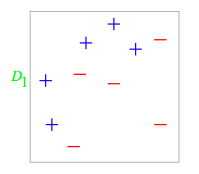
\includegraphics[height=1.1cm]{fig/0} & 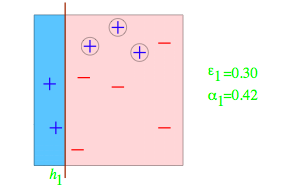
\includegraphics[height=1.1cm]{fig/1} & \multirow{3}{*}{$\to$} & \multirow{3}{*}{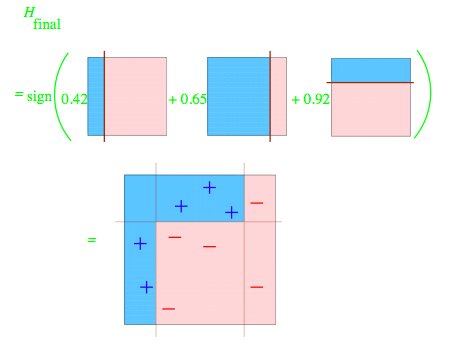
\includegraphics[height=3cm]{fig/6}} \\
        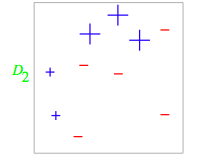
\includegraphics[height=1.1cm]{fig/2} & 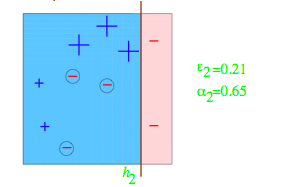
\includegraphics[height=1.1cm]{fig/3} & & \\
        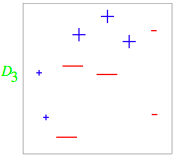
\includegraphics[height=1.1cm]{fig/4} & 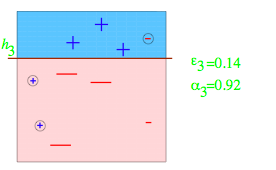
\includegraphics[height=1.1cm]{fig/5} & &
    \end{tabular} 
    \caption{Illustration du fonctionnement d'un algorithme de boosting sur un problème de classification binaire}
    \label{fig:exemple}
\end{figure}    

\paragraph{}
Le premier algorithme de boosting a été développé par \bsc{Schapire} en 90 \cite{schapire1990strength} pour répondre à une question de \bsc{Kearns} \cite{kearns1988thoughts}~: est-il possible de rendre aussi bon que souhaité un algorithme d’apprentissage \og{}faible\fg{}~?
\bsc{Schapire} montra qu'il est toujours possible d'améliorer la performance d'un algorithme faible en l'entraînant sur un ensemble d'exemples bien choisis.
Fort de ces résultats, il a poursuivi ses travaux avec \bsc{Freund} et mis au point en 1995 un algorithme de classification binaire, devenu la référence des algorithmes de boosting~: AdaBoost \cite{freund1995desicion}.
Cet algorithme a servi de base à beaucoup d'autres, parmi lesquels RankBoost \cite{freund1998efficient}, un algorithme utilisé pour résoudre des problèmes de Ranking.

%%%%%%%%%%%%%%%%%%%%%%%%%%%%%%%%%%%%%%%%%%%%%%%%%%%%%%%%%%%%%%%%%%%%%%%%%%%%%%%

\section{AdaBoost}

Adaboost est l'algorithme le plus populaire de la famille du boosting. Il est essentiellement utilisé pour résoudre des problèmes de classification binaire. Trois idées fondamentales sont à la base d'Adaboost~:
\begin{enumerate}
    \item l'utilisation d'un comité d'experts spécialisés (hypothèses faibles $h_t$) que l'on fait voter pour atteindre une décision $H$
    \item la pondération adaptative $\alpha_t$ des votes en fonction du taux d'erreur de chaque expert
    \item la modification de la distribution $D$ des exemples disponibles pour entraîner chaque expert, en surpondérant au fur et à mesure les exemples mal classés aux itérations précédentes
\end{enumerate}

\begin{algorithm}
    \caption{AdaBoost}
    \label{alg:adaboost}
    \begin{algorithmic}
        %%-----------------------------------------------
        \REQUIRE un ensemble d'apprentissage 
                 $\mathcal{S} = \{ (\vs{x}_{1},y_{1}),\ldots,(\vs{x}_{m},y_{m}) \}$\\
                 avec $y_{i} \in \{+1, -1\}, i = 1, \dots, m$,\\
            le nombre d'itérations $T$,\\
            la distribution initiale $D : D(i) = \frac{1}{m}, i=1,\ldots,m$,\\
            un algorithme d'apprentissage faible \emph{WeakLearn}
        \ENSURE l'hypothèse finale $H(\vs{x}) = sign(\sum_{t=1}^{T} \alpha_{t} h_{t}(\vs{x}))$

        %\STATE Initialiser la distribution $D$~: $D_1(i) = \frac{1}{m}, i=1,\ldots,m$   %$D_1 \leftarrow D$
        \STATE Initialiser la distribution $D_1 \leftarrow D$ %   D_1 \leftarrow D$
        %\STATE Initialiser la distribution de probabilité des exemples $D_1(i) = \frac{1}{m}, i=1,\ldots,m$%$D_1 \leftarrow D$

        \FOR{$t = 1$ to $T$}
            \STATE Tirer un échantillon d'apprentissage $\mathcal{S}_t$ dans $\mathcal{S}$ selon $D_t$
            \STATE Trouver une \emph{hypothèse faible} $h_t$ qui minimise l'erreur $\epsilon_t$ sur $\mathcal{S}_t$
            \STATE Calculer le poids $\alpha_t$ de $h_t$~:
                   typiquement $\alpha_t \leftarrow \frac{1}{2}\textrm{ln}\frac{1 - \epsilon_t}{\epsilon_t}$ 

            \FORALL{$i = 1, \dots, m$}
                \STATE Mettre à jour la distribution de probabilité de l'exemple $\vs{x}_i$~:\\
                       $D_{t+1}(i) \leftarrow \frac{ D_t(i) \, e^{- \alpha_t y_i h_t(\vs{x}_i)} }{ Z_t }$, 
                       avec $Z_t$ un facteur de normalisation
            \ENDFOR

            \STATE $t \leftarrow t + 1$

        \ENDFOR

        %\STATE Retourner l'hypothèse finale~: $H(\vs{x}) = sign(\sum_{t=1}^{T} \alpha_{t} h_{t}(\vs{x}))$
        %%-----------------------------------------------
    \end{algorithmic}
\end{algorithm}

%%%%%%%%%%%%%%%%%%%%%%%%%%%%%%%%%%%%%%%%%%%%%%%%%%%%%%%%%%%%%%%%%%%%%%%%%%%%%%%

\section{RankBoost}

L'algorithme Rankboost -- qui est l'objet de l'article étudié ici -- ne traite pas les problèmes de classification comme Adaboost mais les problèmes de \emph{ranking}.
Dans ce type de problèmes, on cherche à ordonner un ensemble d’instances $\mathcal{X} = \{x_0, \dots, x_m\}$ les unes par rapport aux autres en leur donnant un \emph{rang}. C'est la fonction $H : \mathcal{X} \to \mathbb{R}$ qui définit le rang de chaque instances.
Cette fonction est apprise à partir d'un ensemble de \emph{caractéristiques} $\mathcal{F} = \{f_0, \dots, f_n \}$ avec $f_i(x_0) > f_i(x_1)$ si \og{}la caractéristique $i$ préfère $x_0$ à $x_1$\fg{} et $f_i(x) = \phi$ si $x$ ne peut pas être classé selon $f_i$.
Nous verrons par la suite que ces fonctions servent de base à l'algorithme d'apprentissage faible générant les \emph{hypothèses faibles} $h_t$.

\paragraph{}
La relation d'ordre à approximer est définie par la fonction de \emph{feedback} $\Phi : \mathcal{X} \times \mathcal{X} \to \mathbb{R}$.
$\Phi(x_0, x_1)$ traduit le degré suivant lequel l'instance $x_1$ est préféré à $x_0$~:
\[
    \left\{
    \begin{tabular}{lcl}
          $\Phi(x_0, x_1) > 0$  & si &  $x_1 \succ x_0$ \\
          $\Phi(x_0, x_1) < 0$  & si &  $x_0 \succ x_1$ \\
          $\Phi(x_0, x_1) = 0$  & si &  $x_0 \sim  x_1$
    \end{tabular}
    \right.
\]
avec $\Phi(x, x) = 0$ $\forall x \in \mathcal{X}$ et $\Phi(x_0, x_1) = -\Phi(x_1, x_0)$ $\forall x_0,x_1 \in \mathcal{X}^2$ (la transitivité n'est pas assurée).

\paragraph{}
La fonction de feedback $\Phi$ et les caractéristiques $f_i$ sont données en entrée de l'algorithme Rankboost et servent à construire l'hypothèse finale $H$.

\paragraph{}
Les couples d'instances sont pondérés par une distribution de probabilité où tous les poids négatifs sont annulés et donc ignorés (la matrice $\Phi$ est antisymétrique et les poids négatifs n'apportent aucune information supplémentaire)~:
\[
    D(x_i, x_j) = c . max(0, \Phi(x_i, x_j))
\]
avec $c$ une constante positive de normalisation telle que
\[
    \sum_{x_0,x_1} D(x_0, x_1) = 1
\]
Comme pour AdaBoost, la distribution $D$ permet de se concentrer sur les paires d'instances mal ordonnées par les hypothèses construites au cours des itérations précédentes.

\paragraph{}
Le but de l'algorithme Rankboost est de trouver une hypothèse forte $H$ qui minimise le critère \emph{rloss} suivant $D$
\[
    \text{rloss}_D(H) = \sum_{x_0, x_1} D(x_0, x_1) [H(x_1) \leq H(x_0)]
\]
où $[H(x_1) \leq H(x_0)]$ vaut 1 si $H(x_1) \leq H(x_0)$ est bien prédit et 0 sinon. % \llbracket \ldbrack 

\begin{algorithm}
    \caption{RankBoost}
    \label{alg:rankboost}
    \begin{algorithmic}
        %%-----------------------------------------------
        \REQUIRE ~\\
            la fonction de feedback $\Phi$,\\
            un ensemble de \emph{caractéristiques} $\mathcal{F} = \{f_0, \dots, f_n \}$,\\
            le nombre d'itérations $T$,\\
            la distribution initiale $D$,\\
            un algorithme d'apprentissage faible \emph{WeakLearn}
        \ENSURE l'hypothèse finale $H(\vs{x}) = \sum_{t=1}^{T} \alpha_t h_t(\vs{x})$%$H$

        \STATE Initialiser la distribution $D_1 \leftarrow D$ %   D_1 \leftarrow D$

        \FOR{$t = 1$ to $T$}
%            \STATE Tirer un échantillon d'apprentissage $\mathcal{S}_t$ dans $\mathcal{S}$ selon $D_t$
            \STATE Apprendre une \emph{hypothèse faible} $h_t : \mathcal{X} \to \mathbb{R}$ avec \emph{WeakLearn}% qui maximise $r_t$\\
%                   avec $r_t = \underset{\vs{x}_i, \vs{x}_j}{\sum} D_t(\vs{x}_i, \vs{x}_j) (h_t(\vs{x}_j) - h_t(\vs{x}_i))$ 
            \STATE Calculer le poids $\alpha_t \in \mathbb{R}$ de $h_t$%~:
%                   $\alpha_t \leftarrow \frac{1}{2}\textrm{ln}\frac{1 + r_t}{1 - r_t}$

            \FORALL{$i = 1, \dots, m$}
                \FORALL{$j = 1, \dots, m$}
                    \STATE Mettre à jour la distribution de probabilité du couple $(\vs{x}_i, \vs{x}_j)$~:\\
                           $D_{t+1}(\vs{x}_i, \vs{x}_j) \leftarrow
                           \frac{ D_t(\vs{x}_i, \vs{x}_j) \, \exp( \alpha_t (h_t(\vs{x}_i) - h_t(\vs{x}_j))) }{ Z_t }$\\
                           avec $Z_t$ un facteur de normalisation
                \ENDFOR
            \ENDFOR

            \STATE $t \leftarrow t + 1$

        \ENDFOR

        %\STATE Retourner l'hypothèse finale~: $H(\vs{x}) = \sum_{t=1}^{T} \alpha_t h_t(\vs{x})$
        %%-----------------------------------------------
    \end{algorithmic}
\end{algorithm}

\paragraph{}
Pour minimiser le critère \emph{rloss}, nous devons construire à chaque itération une hypothèse $h_t$ de sorte à minimiser
\[
    Z_t = \sum_{x_0, x_1} D_t(x_0, x_1) \exp(\alpha_t(h_t(x_0) - h_t(x_1)))
\]
ce qui revient à maximiser la valeur $|r_t|$ avec
\[
    r_t = \sum_{x_0, x_1} D_t(x_0, x_1) (h_t(x_0) - h_t(x_1))
\]
et à définir $\alpha_t$ tel que
$
    \alpha_t = \frac{1}{2} \ln \left( \frac{1+r_t}{1-r_t} \right)
$
si $h_t : \mathcal{X} \to [0, 1]$.

\paragraph{}
La méthode la plus simple et la plus évidente pour construire les hypothèses faibles $h_t$ serait de les définir comme des \emph{caractéristiques} $f_i$, avec une valeur par défaut $q_\text{def}$ attribuée aux instances non évaluées.
Mais combiner plusieurs \emph{caractéristiques} peut s’avérer difficile, car toutes n’utilisent pas forcément la même échelle de notes. 
Afin de tenir compte uniquement de la relation d'ordre, les hypothèses faibles sont définies de la façon suivante~:
\[
    h(x) = 
    \left\{
    \begin{tabular}{lcl}
          1                 & si & $f_i(x)  >   \theta$ \\
          0                 & si & $f_i(x) \leq \theta$ \\
          $q_{\text{def}}$  & si & $f_i(x)  =   \phi$
    \end{tabular}
    \right.
    \text{ avec } \theta \in \mathbb{R} \text{ et } q_{\text{def}} \in \{0, 1\}
\]
Ainsi, à chaque itération $t$ de l'algorithme, l'hypothèse faible $h_t$ est construite en choisissant une \emph{caractéristique} dans $\mathcal{F}$, un seuil $\theta$ et une valeur par défaut $q_{\text{def}}$ de sorte à maximiser $r_t$.

%%%%%%%%%%%%%%%%%%%%%%%%%%%%%%%%%%%%%%%%%%%%%%%%%%%%%%%%%%%%%%%%%%%%%%%%%%%%%%%

\section{Résultats}

Les performances de Rankboost sont évaluées à travers deux problèmes. Pour des raisons de place, nous ne détaillerons que le second~:
%Les performances de Rankboost sont évaluées à travers deux problèmes~:
%\begin{itemize}
%    \item l'agglomération intelligente de plusieurs stratégies de recherche d'informations sur le web
%    \item la création d'un système de recommandation collaboratif de films (ie. basé sur les préférences d'autres utilisateurs)
%\end{itemize}
%
%\paragraph{}
%Pour des raisons de place, nous ne détaillerons que le second problème qui consiste à conseiller un \emph{utilisateur cible}, Bob, sur de nouveaux films qu'il a de grandes chances d'aimer. 
la création d'un système de recommandation collaboratif de films pour un \emph{utilisateur cible}, Bob.%, sur de nouveaux films qu'il a de grandes chances d'aimer. 

\paragraph{}
Le principe est le suivant~:
\begin{itemize}
    \item le système demande à Bob d'évaluer une liste de films qu'il a déjà vu;
    \item les notes attribuées par les autres utilisateurs de la base sont examinées et utilisées pour retourner une liste de nouveaux films supposés plaire à Bob;
    \item on s'intéresse aux utilisateurs dont les préférences sont similaires à celles de Bob et on combine leurs recommandations sur les films qu'il n'a pas encore vu.
\end{itemize}
Les données utilisées sont tirées de la base \emph{EachMovie}\footnote{\url{http://www.research.digital.com/SRC/eachmovie/}} de \emph{Digital Equipement Corporation}.

\paragraph{}
Dans cet expérience, les \emph{instances} sont des films et $\mathcal{X}$ représente l'ensemble de tous les films connus par le système.

Les \emph{caractéristiques} $f_i(x)$ correspondent aux notes accordées par l'utilisateur $i$ sur le film $x$ ($f_i(x) = \phi$ si le film $x$ n'a pas été évalué par l'utilisateur $i$). Ainsi, $f_i(x_1) > f_i(x_0)$ si l'utilisateur $i$ a préféré le film $x_1$ au film $x_0$. Les notes sont prises dans l'ensemble $R = \{0.0, 0.2, 0.4, 0.6, 0.8, 1.0\}$.

La fonction de \emph{feedback} $\Phi$ traduit les préférences de Bob. % (ie. celui pour qui on veut faire la recommandation de films).
$\Phi(x_0, x_1) = 1$ si il préfère le film $x_1$ au film $x_0$ et $-1$ dans le cas contraire.
Si Bob n'est pas capable de discriminer les deux films (ie. si il ne les a pas tous vus ou si il n'a pas de préférence) alors $\Phi(x_0, x_1) = 0$.

L'hypothèse forte $H : \mathcal{X} \to \mathbb{R}$ attribue un rang aux films. Elle est censé représenter les préférences de Bob sur tous les films, y compris (et surtout) sur ceux qu'il n'a pas vu. $H(x_1) > H(x_0)$ si il est supposé préférer $x_1$ à $x_0$.

\paragraph{}
Les performances de Rankboost sur cette expérience sont mesurées à deux autres algorithmes (l'algorithme du \emph{plus proche voisin} et un algorithme de régression), suivant quatre critères d'évaluation (voir l'article pour plus de détails).
Rankboost obtient les meilleurs résultats sur ces quatre critères.

%%%%%%%%%%%%%%%%%%%%%%%%%%%%%%%%%%%%%%%%%%%%%%%%%%%%%%%%%%%%%%%%%%%%%%%%%%%%%%%

\section{Conclusion et critiques}

Le boosting est une méthode populaire qui permet d'améliorer sensiblement les performances dès lors que l'hypothèse faible est bien choisie.
Il est d'autant plus intéressant qu'il offre des garanties théoriques sur l'erreur en généralisation et qu'il ne nécessite pas de connaissance à priori sur l'algorithme d'apprentissage \og{}faible\fg{} utilisé.

\paragraph{}
Une des principales faiblesses du boosting est sa sensibilité au bruit car les exemples aberrants (\emph{outliners}) obtiennent un poids exponentiellement grand lors de l'apprentissage. Les performances peuvent être grandement affectées lorsque de nombreux exemples sont bruités.
Bien utilisé, ce phénomène peut toutefois devenir une force car il permet de détecter facilement les exemples aberrants.

\paragraph{}
Malgré les qualités discernables de Rankboost, on peut émettre quelques réserves quand à l'évaluation des résultats obtenus.
On peut notamment reprocher à Freund et Schapire le choix non justifié et à priori arbitraire de certaines valeurs utilisées pour la mesure de performance (comme le seuil \emph{truly top-rated instances}). Le choix d'algorithmes très simplifiés pour positionner Rankboost face à l'existant mérite également d'être souligné (le \emph{plus proche voisin} au lieu de des \emph{K plus proches voisins}).

%%%%%%%%%%%%%%%%%%%%%%%%%%%%%%%%%%%%%%%%%%%%%%%%%%%%%%%%%%%%%%%%%%%%%%%%%%%%%%%%

%\bibliographystyle{plain}
\bibliographystyle{alpha}
\bibliography{article}

\end{document}
